% --------------------------
% ---- DECLARE PACKAGES ----
% --------------------------
\documentclass[a4paper, oneside, openright]{book}
\usepackage[T1]{fontenc} % Font encoding, T1 = it
\usepackage{lmodern}
\usepackage{multicol} % Per il frontespizio
\usepackage[utf8]{inputenc} % Input encoding - per caratteri particolari
\usepackage[english]{babel} % Lingua principale italiano, con parti in inglese
\usepackage{blindtext} % Per la generazione di paragrafi lorem ipsum
\usepackage{graphicx} % Per includere immagini esterne
\usepackage[a4paper,top=2.5cm,bottom=2.5cm,left=3cm,right=3cm]{geometry} %impaginazione e margini documento
\usepackage[fontsize=12pt]{scrextend} %dimensione font
\usepackage{graphicx}
\usepackage[parfill]{parskip} % Disabilita l'indentazione dopo essere andati a capo
% \usepackage[hang,flushmargin]{footmisc} % Disabilita l'indentazione nelle footnotes
\usepackage{titlesec}
\usepackage{float}
\usepackage[font=scriptsize, skip=5pt]{caption} % Spazio tra la caption e l'immagine
\usepackage[backend=biber, style=numeric, backref=true,defernumbers=true]{biblatex}
\usepackage[immediate]{silence}
\WarningFilter[temp]{latex}{Command} % silence the warning
\usepackage{sectsty}
\DeactivateWarningFilters[temp] % So nothing unrelated gets silenced
\usepackage{hyperref} % Rende l'indice cliccabile
\usepackage[justification=centering]{caption} % Per centrare le captions
\usepackage{csquotes} % Dipendenza di babel
\usepackage[bottom]{footmisc} % Posiziona le footnotes alla fine della pagina
\usepackage{tikz}
\usepackage{tabularx}
\usepackage{multicol}
\usepackage{multirow}
\usepackage{lastpage}
\usetikzlibrary{positioning, quotes, arrows.meta, calc}
\usepackage{enumerate, mdwlist}
\usepackage{fancyhdr}
\usepackage{amsthm}
\newtheorem{definition}{Definition}
\newtheorem{lemma}{Lemma}
\newtheorem{teorema}{Theorem}
\usepackage{amsmath,amssymb}
\usepackage{minted}

% Algorithms
\usepackage{algorithm}
\usepackage{algpseudocode}

% \usepackage{todonotes}

% ------------------------
% ---- DOCUMENT SETUP ----
% ------------------------
\pagestyle{plain}
\setlength{\headheight}{20pt}

\raggedbottom % Se la pagina non è completa, lascia lo spazio alla fine

\titleformat{\chapter}[display]
    {\normalfont\huge\bfseries}{\chaptertitlename\ \thechapter}{10pt}{\LARGE}
\titlespacing*{\chapter}{0pt}{0pt}{20pt}
\chaptertitlefont{\fontsize{22pt}{30pt}\selectfont}

\hypersetup{ % Setup dell'aspetto dei link
    colorlinks,
    citecolor=black,
    filecolor=black,
    linkcolor=black,
    urlcolor=black
}

% \renewcommand{\footnoterule}{ % Rende la linea delle footnotes larga tutta la pagina
%   \kern -3pt
%   \hrule width \textwidth height 1pt
%   \kern 2pt
% } 
\renewcommand{\footnotesize}{\fontsize{11pt}{13pt}\selectfont} % Imposta la dimensione del testo delle footnotes
\setlength{\footnotesep}{0.5cm} % Imposta lo spazio fra e singole footnotes
\setlength{\skip\footins}{1.5cm} % Imposta lo spazio fra il corpo e le footnotes

\usepackage[normalem]{ulem}


\DeclareUnicodeCharacter{02BC}{}

% ------------------------
% ---- DOCUMENT START ----
% ------------------------
\addbibresource{bibliography.bib} % Importiamo la bibliografia
\begin{document}
\pagenumbering{roman} 
\begin{titlepage}
\begin{figure}[!htb]
    % \centering
    
\includegraphics[width=4cm]{Immagini/logo 2 unive.png}
\end{figure}

\begin{center}
    % \Large{\textbf{UNIVERSITÀ CA' FOSCARI DI VENEZIA}}
    % \vspace{3mm}
    % \\ \normalsize{DIPARTIMENTO DI SCIENZE AMBIENTALI, INFORMATICA E STATISTICA}
    % \vspace{6mm}
    \vspace{13mm}
    \normalsize{\textbf{Artificial Intelligence and Data Engineering}}
    \vspace{13mm}
    \\ \normalsize{Algorithms for Massive Data}
\end{center}

\vspace{10mm}
\begin{center}
    \LARGE{Project: \textbf{The XBW-Transform for Labeled Trees}}
\end{center}

\vspace*{\fill}

\begin{minipage}[t]{1\textwidth}
    {\normalsize{\textbf{Professor}}{\normalsize\vspace{1mm}
    \\ \normalsize{Nicola Prezza }}} \\ 
        
    {\normalsize{\textbf{Author}}{\normalsize\vspace{1mm}
    \\ \normalsize{Davide Tonetto}\\
    \normalsize{Student ID 884585 }}} \\
\end{minipage}

\begin{flushleft}
    {\normalsize{\textbf{Academic year}}{\normalsize\vspace{1mm}
    \\ \normalsize{2024/2025}}}  
\end{flushleft}

\end{titlepage}
 % PAGINA FRONTESPIZIO
\tableofcontents  % Genera l'indice
% \addcontentsline{toc}{chapter}{\listfigurename}
% \listoffigures
\newpage % Nuova pagna

\fancypagestyle{IHA-fancy-style}{%
  \fancyhf{}% Clear header and footer
  %\fancyhead[LE,RO]{\slshape \rightmark}
  \fancyhead[R]{\slshape \leftmark}
  \fancyfoot[C]{\thepage\ of \pageref{LastPage}}% Custom footer
  \renewcommand{\headrulewidth}{0.4pt}% Line at the header visible
  %\renewcommand{\footrulewidth}{0.4pt}% Line at the footer visible
}

% Redefine the plain page style
\fancypagestyle{plain}{%
  \fancyhf{}%
  \fancyfoot[C]{\thepage\ of \pageref{LastPage}}%
  \renewcommand{\headrulewidth}{0pt}% Line at the header invisible
  \renewcommand{\footrulewidth}{0pt}% Line at the footer visible
}

\pagestyle{IHA-fancy-style}

\pagenumbering{arabic} % Riabilita la numerazione in modo che cominci dal primo capitolo
\setcounter{chapter}{0} % Fa risultare l'introduzione come capitolo 0
% ------------------
% ---- CHAPTERS ----
% ------------------
\chapter{Wheeler Graphs}

\section{Definition of Wheeler Graph}

\begin{definition} \label{def_wheeler_graphs}
    A Wheeler graph $G=(V,E)$ is defined as a directed graph with labeled edges, equipped with a total order $<_{\pi}$ on the nodes in $V$, which satisfies the following three axioms:

    \begin{enumerate}[(i)]
        \item All vertices with in-degree $0$ must precede those with a greater in-degree in the ordering; \label{axiom_1}
    \suspend{enumerate}
    For every pair of edges $(u_1,v_1,k_1)$ and $(u_2,v_2,k_2)$:
    \resume{enumerate}[{[(i)]}]
        \item $k_1<k_2 \Rightarrow v_1<_{\pi}v_2$; \label{axiom_2}
        \item $(k_1=k_2) \wedge (u_1<_{\pi}u_2) \Rightarrow v_1\leq_{\pi}v_2$. \label{axiom_3}
    \end{enumerate}
\end{definition}

\section{Examples of Wheeler Graphs}
\begin{figure}[H]
    \centering
    \begin{tikzpicture}[node distance={25mm}, thick, auto=center, main/.style = {draw, circle}]
        \node[main] (1) {$x_1$};
        \node[main] (2) [below left of=1] {$x_2$};
        \node[main] (3) [below right of=1] {$x_3$};
        \node[main] (4) [below of=2] {$x_4$};
        \node[main] (5) [below of=3]{$x_5$};
        \draw[red, ->] (1) -- (3);
        \draw[red, ->] (1) -- (2);
        \draw[red, ->] (4) -- (3);
        \draw[red, ->] (5) -- (3);
        \draw[green, ->] (2) -- (5);
        \draw[blue, ->] (2) -- (4);
        \draw (4) edge[blue, loop left] (4);
    \end{tikzpicture}
    \caption[Example of a Wheeler Graph]{Example of a Wheeler graph with $\sigma=3$. The label order is as follows: red $<$ blue $<$ green. The resulting total order of nodes is: $x_1<x_2<x_3<x_4<x_5$.}
    \label{fig:wheeler_example}
\end{figure}

Consider Figure \ref{fig:wheeler_example}. Axiom (\ref{axiom_1}) states that nodes with no incoming edges (in-degree $0$) must be positioned at the beginning of the total order and never after nodes with a greater in-degree. In the example, node $x_1$ is the only node with in-degree $0$, so it is placed as the first element in the resulting total order.

\begin{figure}[H]
    \centering
    \begin{tabular}{cc}
        \begin{tikzpicture}[node distance={15mm}, thick, auto=center, main/.style = {draw, circle}]
            \node[main] (1)  {$u_1$};
            \node[main] (2) [right of=1] {$u_2$};
            \node[main] (3) [above of=1] {$v_1$};
            \node[main] (4) [above of=2] {$v_2$};
            \draw[->, red] (1) -- (3);
            \draw[->, blue] (2) -- (4);
        \end{tikzpicture} &
        \begin{tikzpicture}[node distance={15mm}, thick, auto=center, main/.style = {draw, circle}]
            \node[main] (3) {$v$};
            \node[main] (1) [below left of=3] {$u_1$};
            \node[main] (2) [below right of=3] {$u_2$};
            \draw[->, red] (1) -- (3);
            \draw[->, blue] (2) -- (3);
        \end{tikzpicture} \\
        (a) & (b) \\
    \end{tabular}
    \caption{Examples for Axiom (\ref{axiom_2}).}
    \label{fig:example_axiom_2}
\end{figure}

To better understand Axiom (\ref{axiom_2}), consider Figure \ref{fig:example_axiom_2}. In example (a), we have two edges $(u_1,v_1,red)$ and $(u_2,v_2,blue)$ with $red<blue$. According to the axiom, since the edges have different labels, the destination node of the edge with the smaller label (in this case $v_1$) must precede the destination node of the edge with the larger label, so we obtain $v_1$ before $v_2$ in the total order.

In example (b), we instead have two edges $(u_1,v,red)$ and $(u_2,v,blue)$ with $red<blue$, but they share the same destination node. This case is not accepted by the second axiom because, if the labels are different, their order must be reflected in the destination nodes, which thus cannot be the same.

\begin{figure}[H]
    \centering
    \begin{tabular}{cc}
        \begin{tikzpicture}[node distance={15mm}, thick, auto=center, main/.style = {draw, circle}]
            \node[main] (1)  {$u_1$};
            \node[main] (2) [right of=1] {$u_2$};
            \node[main] (3) [above of=1] {$v_1$};
            \node[main] (4) [above of=2] {$v_2$};
            \draw[->, red] (1) -- (3);
            \draw[->, red] (2) -- (4);
        \end{tikzpicture} &
        \begin{tikzpicture}[node distance={15mm}, thick, auto=center, main/.style = {draw, circle}]
            \node[main] (3) {$v$};
            \node[main] (1) [below left of=3] {$u_1$};
            \node[main] (2) [below right of=3] {$u_2$};
            \draw[->, red] (1) -- (3);
            \draw[->, red] (2) -- (3);
        \end{tikzpicture} \\
        (a) & (b) \\
    \end{tabular}
    \caption{Examples for Axiom (\ref{axiom_3}).}
    \label{fig:example_axiom_3}
\end{figure}

To better understand Axiom (\ref{axiom_3}), consider Figure \ref{fig:example_axiom_3}. In example (a), we have two edges $(u_1,v_1,red)$ and $(u_2,v_2,red)$ with $u_1<u_2$. The axiom applies here because the edges share the same label. Consequently, the order of the source nodes propagates to the destination nodes of the two edges. Specifically, the destination node of the edge whose source node is smaller in the total order must not be larger than the destination node of the edge whose source node is larger. In this case, since $u_1<u_2$, we obtain $v_1\leq v_2$.

In example (b), we consider the case where the two edges $(u_1,v,red)$ and $(u_2,v,red)$ with $u_1<u_2$ have the same label and share the same destination node. Again, the axiom applies, requiring that $v_1\leq v_2$. In this case, we obtain $v_1=v_2$.

\section{Properties of Wheeler Graphs}
The following is a list of some properties of Wheeler graphs that can be derived from the axioms (Definition \ref{def_wheeler_graphs}).

\begin{lemma} \label{property_1}
    All incoming edges to a node $v$ must have the same label. This property makes it equivalent to label either the nodes or the edges of the graph.
\end{lemma}

\begin{proof}
    Lemma \ref{property_1} is a natural derivation of the second Wheeler axiom (Definition \ref{def_wheeler_graphs}). It states that given two edges $(u_1,v_1,k_1)$ and $(u_2,v_2,k_2)$ with $k_1<k_2$, the order of the edge labels propagates to the destination nodes, implying $v_1<v_2$. This means that the destination nodes $v_1$ and $v_2$ cannot be the same if they receive incoming edges with different labels; otherwise, the considered graph would not be Wheeler.
\end{proof}

\begin{lemma} \label{property_2}
    A node $v$ may have multiple outgoing edges with the same label.
\end{lemma}

\begin{proof}
    Assume, for contradiction, that the statement does not hold and that a node $v$ cannot have multiple outgoing edges with the same label if the graph is Wheeler. The graph in Figure \ref{fig:wheeler_example} is a valid counterexample demonstrating the opposite, as node $x_1$ has two outgoing edges labeled $red$, and the graph is Wheeler. This leads to a contradiction.
\end{proof}

\begin{lemma} \label{property_3}
    Consider a Wheeler graph $G=(V,E)$ with labeling defined over a set $\Sigma=\{a,b,c\}$, where the label order is $a<b<c$. Let $V_a \subseteq V$ be the set of vertices with label $a$ (i.e., those with incoming edges labeled $a$), $V_b \subseteq V$ the set of vertices with label $b$, and $V_c \subseteq V$ the set of vertices with label $c$. Also, let $u_a \in V_a$, $u_b \in V_b$, and $u_c \in V_c$. Then, in the context of vertex ordering in the graph, it holds that $u_a < u_b < u_c$. More generally, all vertices in $V_k$ for a certain label $k$ will be consecutive in the ordering, with no nodes of other labels interspersed among them in the total order.
\end{lemma}

\begin{proof}
    Lemma \ref{property_3} follows naturally from the second Wheeler axiom (Definition \ref{def_wheeler_graphs}). Consider a Wheeler graph $G=(V,E)$ with labeling over a set $\Sigma=\{a,b\}$, where the order of labels is $a<b$. Let $V_a \subseteq V$ be the set of vertices labeled $a$ and $V_b \subseteq V$ be the set of vertices labeled $b$. Suppose, for contradiction, that there exist two nodes $u_a \in V_a$ and $u_b \in V_b$ such that $u_b < u_a$ in the Wheeler ordering.
    
    Since $u_a \in V_a$ and $u_b \in V_b$, by the definition of sets $V_a$ and $V_b$, there must exist two edges $(v_1, u_a, a)$ and $(v_2, u_b, b)$. However, this leads to a contradiction because the second axiom states that for two edges $(u_1,v_1,k_1)$ and $(u_2,v_2,k_2)$ with $k_1<k_2$, the order of edge labels must be reflected in the destination nodes, meaning $v_1<v_2$. In our case, $a<b$, but $u_b < u_a$, implying the graph is not Wheeler.
\end{proof}

\begin{lemma} \label{property_4}
    Consider a total Wheeler order. Let $V_k$ be the set containing all nodes with the same label $k$. Let $V_k^1$ and $V_k^2$ be two partitions of $V_k$, where $V_k^1$ contains all nodes $v_1$ with incoming edges from nodes preceding $v_1$ in the total order, while $V_k^2$ contains all nodes $v_2$ with incoming edges from nodes following $v_2$ in the total order. Consequently, the intersection of $V_k^1$ and $V_k^2$ contains at most one vertex $u$, and all vertices in $V_k^1 \setminus \{u\}$ precede those in $V_k^2$ in the ordering. Moreover, given a vertex $v \in V_k^1$, there cannot exist an edge $(v, z, k)$ with $z<v$, and similarly, given a vertex $v \in V_k^2$, there cannot exist an edge $(v, z, k)$ with $z>v$ (see \cite{inapproximabilityWheelerGraphs}).
\end{lemma}

\subsection{Path Coherence}
The following defines \textit{path coherence} and a related property of Wheeler graphs introduced and proven in \cite{wheelerGrpahs}.

\begin{definition}[Path Coherence]
    A labeled directed graph $G$ is said to be \textit{path coherent} if there exists a total order of nodes such that, for every consecutive interval $[i, j]$ of nodes and a string $\alpha$, the nodes reachable from those in $[i, j]$ in $|\alpha |$ steps, following edges whose labels form $\alpha$ when concatenated, themselves form an interval in the total order.
\end{definition}

\begin{lemma} \label{property_5}
    A Wheeler graph is path coherent with respect to any possible Wheeler order of the nodes.
\end{lemma}

Thanks to this crucial property, it was proven in \cite{wheelerGrpahs} that if the state diagram of a finite-state automaton is a Wheeler graph, then, due to Lemma \ref{property_5}, the nodes can be ordered so that for any string, the nodes reachable from the initial state(s) by processing that string are consecutive. This means that even if the automaton is non-deterministic, it can still be stored compactly and used to process strings efficiently.

\subsection{Topological Ordering for \texorpdfstring{$\sigma=1$}{Lg}}
The following defines \textit{topological ordering} and a related property of Wheeler graphs introduced and proven in \cite{inapproximabilityWheelerGraphs}.

\begin{definition}[Topological Ordering]
    A topological ordering is a linear ordering of all vertices of a directed graph. The nodes of a graph are said to be topologically ordered if they are arranged such that each node precedes all nodes connected to its outgoing edges. The topological ordering of a graph may not be unique. In the worst case, there can be $n!$ different topological orderings corresponding to all possible permutations of the $n$ nodes. A topological ordering is possible if and only if the graph has no directed cycles, meaning it is a directed acyclic graph (DAG) \cite{topol16ogicalOrdering}.
\end{definition}

\begin{lemma} \label{property_6}
    For $\sigma=1$, every Wheeler order also represents a topological ordering, except for vertices with self-loops, which must be placed at the end of the order since a cyclic graph cannot have a valid topological ordering.
\end{lemma}

This property follows from Lemma \ref{property_4} and the first axiom (Definition \ref{def_wheeler_graphs}). Finally, it is important to highlight that this result is used in \cite{inapproximabilityWheelerGraphs} to prove that the Wheeler graph recognition problem can be solved in linear time when $\sigma=1$.

\begingroup
\sloppy
\raggedright
\section{Bipartite Representation of Wheeler Graphs} \label{rapp_bipartita}
\endgroup
The following section explains a simple and intuitive technique used to graphically check whether a directed labeled graph, along with its total node ordering, satisfies the three Wheeler axioms (Definition \ref{def_wheeler_graphs}). More specifically, the technique involves representing the graph as a bipartite graph with useful properties related to the three Wheeler axioms. Additionally, later in the text, we will see how this idea is also useful for the Wheelerization problem of a graph.

\subsection{Construction of the Bipartite Graph}
Consider a directed labeled graph on the edges $G=(V,E)$ where $V=\{x_1,\dots,x_n\}$ and a total ordering of $V$ (in the example, consider $x_1<x_2<\dots<x_n$). The bipartite graph $B=(V_1,V_2,E_B)$ is constructed as follows:

\begin{itemize}
    \item $V_1=\{x_i^s : i \in [1, n]\}$. Where the node $x_i^s \in V_1$ corresponds to the node $x_i \in V$ for $1 < i < n$. This set is thus composed of the nodes in $V$, and is ordered according to the given ordering.
    \item $V_2=\{x_i^d : i \in [1, n]\}$. Where the node $x_i^d \in V_2$ corresponds to the node $x_i \in V$ for $1 < i < n$. This set is also composed of the nodes in $V$, and is ordered according to the given ordering.
    \item $E_B=\{(u, v) : u \in V_1 \wedge v \in V_2 \wedge (u,v) \in E\}$. Therefore, for every edge $(x_i,x_j) \in E$, a corresponding edge is created in the bipartite graph such that $x_i = x_i^s \in V_1$ and $x_j=x_j^d \in V_2$ with $i, j \in [1, n]$. For example, given the edge $(x_1, x_4)$, an edge is created between $x_1^s$ and $x_4^d$ (edge $(x_1^s,x_4^d)$ in the bipartite graph).
\end{itemize}

The following explanation assumes a vertical construction of the bipartite graph. As a result, since the nodes in $V_1$ and $V_2$ are ordered according to the total ordering of $V$ (in the example, we have $x_1^s<x_2^s<\dots<x_n^s$ and $x_1^d<x_2^d<\dots<x_n^d$), a node $x_i^s \in V_1$ is positioned graphically above a node $x_j^s \in V_1$ if and only if $i < j$ in the ordering, and similarly, a node $x_i^d \in V_2$ is positioned graphically above a node $x_j^d \in V_2$ if and only if $i < j$ in the ordering.

This vertical construction implies that the nodes in the set $V_1$ will be arranged in ascending order downward, maintaining the total ordering. Similarly, the nodes in the set $V_2$ will be arranged in ascending order downward, respecting the established ordering. In this way, the vertical position of the nodes reflects the ordering of the nodes within the graph. See the example in Figure \ref{fig:bipartite_example}-(a), which shows the bipartite representation of the graph in Figure \ref{fig:wheeler_example}.

\subsection{Properties of the Bipartite Graph}
As introduced earlier, the bipartite representation allows us to easily verify whether the three Wheeler axioms (Definition \ref{def_wheeler_graphs}) are satisfied by the graph $G$ and the ordering on $V$ (consider the graph and ordering defined in the previous section). The properties related to the axioms are as follows:
\begin{itemize}
    \item Axiom (\ref{axiom_1}) is satisfied if for every pair of nodes $u, v \in V$ it holds that if $indegree(u) = 0 \wedge indegree(v) > 0$, then $u < v$ in the ordering.
    \item Axiom (\ref{axiom_2}) is satisfied if every node in the bipartite graph has all incoming edges with the same label, and moreover, the order of the labels respects the node ordering. Formally, let $\lambda(u)$ be a function that returns the label of a given node $u \in V$. It must hold that $\lambda(x_1) \leq \lambda(x_2) \leq \dots \leq \lambda(x_n)$.
    \item Axiom (\ref{axiom_3}) is satisfied if there are no edges with the same label crossing in the bipartite graph. Formally, a crossing is defined as follows: let $(x_i^s,x_j^d,k_1)$, $(x_k^s,x_w^d,k_2)$ be two edges of the bipartite graph labeled $k_1$ and $k_2$, respectively, a crossing occurs if $(i < k \wedge j > w) \lor (i > k \wedge j < w)$, where the subscripts of the nodes indicate their position in the ordering.
\end{itemize}

\begingroup
\sloppy
\raggedright
\subsection{Examples of Bipartite Representation of Wheeler Graphs}
\endgroup
Consider the Wheeler graph shown in Figure \ref{fig:wheeler_example}, and the resulting bipartite graph shown in Figure \ref{fig:bipartite_example}-(a). 

\begin{figure}[H]
    \centering
    \begin{tabular}{cc}
        \begin{tikzpicture}[node distance={15mm}, thick, auto=center, main/.style = {draw, circle}] 
            \node[main] (1s) {$x_1^s$};
            \node[main] (2s) [below of=1s] {$x_2^s$}; 
            \node[main] (3s) [below of=2s] {$x_3^s$};
            \node[main] (4s) [below of=3s] {$x_4^s$};
            \node[main] (5s) [below of=4s] {$x_5^s$};
            \node[main] (1d) [right=2cm of 1s] {$x_1^d$};
            \node[main] (2d) [below of=1d] {$x_2^d$}; 
            \node[main] (3d) [below of=2d] {$x_3^d$};
            \node[main] (4d) [below of=3d] {$x_4^d$};
            \node[main] (5d) [below of=4d] {$x_5^d$};
            \draw[red, ->] (1s) -- (3d);
            \draw[red, ->] (1s) -- (2d);
            \draw[red, ->] (4s) -- (3d);
            \draw[red, ->] (5s) -- (3d);
            \draw[green, ->] (2s) -- (5d);
            \draw[blue, ->] (2s) -- (4d);
            \draw[blue, ->] (4s) -- (4d);
        \end{tikzpicture} &
        \begin{tikzpicture}[node distance={15mm}, thick, auto=center, main/.style = {draw, circle}] 
            \node[main] (3s) {$x_3^s$};
            \node[main] (2s) [below of=3s] {$x_2^s$}; 
            \node[main] (1s) [below of=2s] {$x_1^s$};
            \node[main] (4s) [below of=1s] {$x_4^s$};
            \node[main] (5s) [below of=4s] {$x_5^s$};
            \node[main] (3d) [right=2cm of 3s] {$x_3^d$};
            \node[main] (2d) [below of=3d] {$x_2^d$}; 
            \node[main] (1d) [below of=2d] {$x_1^d$};
            \node[main] (4d) [below of=1d] {$x_4^d$};
            \node[main] (5d) [below of=4d] {$x_5^d$};
            \draw[red, ->] (1s) -- (3d);
            \draw[red, ->] (1s) -- (2d);
            \draw[red, ->] (4s) -- (3d);
            \draw[red, ->] (5s) -- (3d);
            \draw[green, ->] (2s) -- (5d);
            \draw[blue, ->] (2s) -- (4d);
            \draw[blue, ->] (4s) -- (4d);
        \end{tikzpicture} \\
        (a) & (b) \\
    \end{tabular}
    \caption[Bipartite Representation of a Wheeler Graph]{Example of bipartite representation of the graph in Figure \ref{fig:wheeler_example}, useful for verifying that it satisfies the three Wheeler axioms. (a) respects the correct ordering, while (b) does not.}
    \label{fig:bipartite_example}
\end{figure}

As we can observe, the three axioms are satisfied, because:
\begin{itemize}
    \item $x_1$ is the only node with in-degree $0$ and is at the beginning of the ordering;
    \item all nodes have all incoming edges with the same label\footnote{In the image, the colors represent the labels.};
    \item starting from the top, the sequence of labels assigned to the incoming edges on each node is as follows: red, red, blue, green, which respects the ordering of the alphabet considered (red $<$ blue $<$ green);
    \item there are no crossings between edges with the same color in the bipartite graph.
\end{itemize}
Therefore, we can confidently assert that the graph in question is a Wheeler graph for the given node order.

The example in Figure \ref{fig:bipartite_example}-(b), however, is constructed using the graph from Figure \ref{fig:wheeler_example}, but considering the following node order: $x_3<x_2<x_1<x_4<x_5$. The resulting bipartite graph shows that the graph from Figure \ref{fig:wheeler_example} with the order $x_3<x_2<x_1<x_4<x_5$ is not a Wheeler graph, because:
\begin{itemize}
    \item the first axiom is not satisfied since node $x_1$ is not at the beginning of the ordering;
    \item the third axiom is not satisfied because there are red edges that cross in the bipartite graph.
\end{itemize}
\newpage
\
\newpage
\chapter{Extended Burrows-Wheeler Transform}
\section{Introduction} 

The Extended Burrows-Wheeler Transform (XBWT) is a data structure designed to efficiently compress and index labeled trees. A labeled tree is a data structure where each node is assigned a label from a given alphabet, and the tree can have an arbitrary shape and degree.

XBWT works by linearizing a labeled tree into two coordinated arrays: one capturing the structural properties of the tree and the other storing its labels. This transformation allows for efficient representation, navigation, and querying of the tree. The key advantage of XBWT lies in its ability to compress labeled trees while supporting a wide range of operations, such as parent-child navigation and sophisticated path-based searches, in (near-)optimal time and space.

One of the primary applications of XBWT is in the compression and indexing of hierarchical data formats, such as XML documents. It provides significant improvements in both compression ratio and query performance compared to traditional tools, making it an invaluable resource for data-intensive applications in fields like bioinformatics, information retrieval, and big data analytics.

This project aims to implement the XBWT data structure and explore its applications in the context of labeled trees. We will start by providing an overview of the theoretical foundations of the XBWT. Finally, we will describe and compare the algorithms for constructing the XBWT and demonstrate its use in compressing and indexing labeled trees.

Let's start with a quick overview of the XBWT and its theoretical foundations.


\subsubsection{How XBWT Works}
The transformation process of XBWT is as follows:
\begin{enumerate}
    \item \textbf{Path Sorting:} The labeled tree is linearized by sorting its nodes based on the \emph{paths} from each node's parent to the root. The resulting order groups nodes with similar upward paths together, clustering related labels.
    \item \textbf{Array Construction:} Two arrays, \( S_{\text{last}} \) and \( S_{\alpha} \), are generated:
    \begin{itemize}
        \item \( S_{\text{last}} \) stores structural information, such as whether a node is the last child of its parent. This encodes the tree’s structure without the need for explicit pointers.
        \item \( S_{\alpha} \) stores the labels of the nodes in the sorted order determined by their upward-path sorting.
    \end{itemize}
    \item \textbf{Compression:} Both \( S_{\text{last}} \) and \( S_{\alpha} \) are highly compressible due to the clustering of similar labels and structural redundancy.
\end{enumerate}

\subsubsection{Key Properties of XBWT}
The XBWT has several key properties that make it an effective tool for labeled tree compression and indexing:
\begin{itemize}
    \item \textbf{Succinctness:} The XBWT representation of a labeled tree uses space close to the \emph{information-theoretic lower bound}, which is \( 2t - \Theta(\log t) + t \log |\Sigma| \) bits for a tree with $t$ nodes and an alphabet of size $|\Sigma|$.
    \item \textbf{Efficient Querying:} XBWT supports a range of navigational operations, such as finding the parent, child, or subtree of a node in near-optimal time.
    \item \textbf{Scalability:} XBWT is particularly useful for large-scale hierarchical data, such as XML documents or phylogenetic trees, where both compression and fast querying are critical.
\end{itemize}

\subsection{Project implementation}

The XBWT data structure will be implemented in C++ using the Succinct Data Structure Library 2.0 (SDSL) for efficient representation and manipulation of compressed data structures. We will develop two algorithms for constructing the XBWT: one efficient linear-time recursive algorithm and one more straightforward iterative algorithm. Also, we will implement the necessary data structures and algorithms for navigating and querying the XBWT, such as parent-child navigation and path-based searches. 

The code is available on GitHub at \url{https://github.com/davide-tonetto-884585/XBWT}. The project will be structured as follows:

\begin{itemize}
    \item \textbf{XBWT.hpp}: File containing the class definition and implementation for the generic XBWT data structure.
    \item \textbf{LabeledTree.hpp}: File containing the class definition and implementation for the generic labeled tree data structure used to feed and test the XBWT.
    \item \textbf{main.cpp}: Main file containing the test cases and examples for the XBWT implementation.
    \item \textbf{experiments.cpp}: File containing the experiments and performance evaluation of the XBWT construction algorithms and compression efficiency.
    \item \textbf{CMakeLists.txt}: CMake configuration file for building the project.
\end{itemize}

The project will be developed and tested on a Linux environment using the GCC compiler and the CMake build system. 

\chapter{Theoretical Background on Labeled Trees}

\section{Labeled Trees}
A \textbf{labeled tree} is a rooted, ordered, hierarchical data structure in which every node is assigned a label from a predefined alphabet $\Sigma$. The structure consists of nodes connected by edges, forming a directed acyclic graph. Formally, a labeled tree $T$ with $t$ nodes can be defined as $T = (V, E, \ell)$, where:
\begin{itemize}
    \item $V$ is the set of nodes,
    \item $E \subseteq V \times V$ is the set of directed edges, and
    \item $\ell: V \to \Sigma$ is a labeling function that assigns a label $\ell(u) \in \Sigma$ to each node $u$.
\end{itemize}

In the case of ordered labeled tree, the children of a node in the tree are ordered, meaning their positions relative to each other matter. A labeled tree can have arbitrary degrees and shapes, and the alphabet $\Sigma$ used for labels can be of arbitrary size.

\subsection{Applications of Labeled Trees}
Labeled trees are widely used in computer science and data representation due to their hierarchical structure and flexibility in modeling relationships. Prominent applications include:
\begin{enumerate}
    \item \textbf{XML Data Representation:} XML documents are often modeled as labeled trees, where each element is a node labeled by its tag, and hierarchical nesting represents parent-child relationships.
    \item \textbf{JSON Data Representation:} JSON objects can be viewed as labeled trees, with keys as labels and values as children.
    \item \textbf{Bioinformatics:} Labeled trees are used to represent phylogenetic trees, genome annotations, and hierarchical clustering.
    \item \textbf{Compiler Design:} Abstract Syntax Trees (ASTs) for programming languages are labeled trees that capture the structure of code.
    \item \textbf{File Systems:} The directory structure of file systems can be viewed as labeled trees.
\end{enumerate}

Efficient representation, navigation, and querying of labeled trees are essential for many applications, motivating the development of specialized data structures and algorithms.

\section{Compressing and Indexing Labeled Trees} \label{compandindexinglabtree}
The goal of compressing and indexing labeled trees is to design a compressed storage scheme for a labeled tree $T$ with $t$ nodes that allows for efficient navigation operations in $T$, as well as fast search and retrieval of subtrees or paths within $T$. To be effective, the compressed representation should minimize the space required to store the tree while supporting a wide range of operations in (near-)optimal time.

Let $u$ be a node in the labeled tree $T$ and let $c \in \Sigma$. We define the following navigation operations on $T$:
\begin{itemize}
    \item \textbf{Navigational queries:} ask for the parent of $u$, the $i$-th child of $u$, or the label of $u$. The last two operations might be restricted to the children of $u$ with a specific label $c$.
    \item \textbf{Path queries:} retrieve the nodes in the subtree rooted at $u$ (any possible order should be implemented).
    \item \textbf{Subpath queries:} ask for the (number of occurrences of) nodes of $T$ that descend from a labeled subpath $P$. Which may be anchored anywhere in the tree (i.e., not necessarily in its root). 
\end{itemize}

A naive solution to index labeled trees is to store the tree in a straightforward manner, such as a list of nodes with their labels and parent-child relationships using pointer in $O(t log t)$. However, this representation is not space-efficient and does not support fast navigation or query operations. 

Many data structures have been proposed to compress and index labeled trees, each with its trade-offs in terms of space usage, query performance, and supported operations. One of the most successful approaches is the Extended Burrows-Wheeler Transform (XBWT), which extends the classical Burrows-Wheeler Transform (BWT) to handle labeled trees efficiently. 

Before the advent of XBWT, Kosaraju \cite{kosaraju1989efficient} proposed a method to index labeled trees by extending the concept of prefix sorting, which is commonly applied to strings, to work with labeled trees by leveraging the structure of tries (prefix trees). To achieve this, he introduced the idea of constructing a suffix tree for a reversed trie allowing subpath queries in $O(|P|\log|\Sigma|+ occ)$ time, where $occ$ is the number of occurrences of $P$ in $T$ but still requiring $O(t \log t)$ space and so not being compressed.

\section{Succinct Data Structures for Trees}
In order to compress the index of labeled trees, we need to avoid the use of pointers and store the tree in a space-efficient manner. Succinct data structures are a class of compressed data structures that support efficient navigation and query operations on the compressed data. These structures are designed to use close to the information-theoretic lower bound on space while providing fast access to the original data. They were first introduced by Jacobson \cite{jacobson1989space} and have been applied to various problems in string processing, graph theory, and data compression.

\subsection{Information-Theoretic Lower Bound for Trees}
The information-theoretic lower bound for storing an unlabeled tree with $t$ nodes is given by:

\begin{itemize}
    \item The number of binary unlabeled trees with $t$ nodes is given by the Catalan number $C_t = \frac{1}{t+1} \binom{2t}{t}$ that can can be approximated as $C_t \approx \frac{4^t}{t^{3/2}\sqrt{\pi}}$ using Stirling's approximation.
    \item The entropy (or the information-theoretic minimum number of bits to encode the structure of the tree) is the logarithm (base 2) of the total number of trees, which is $-\log_2 C_t \approx 2t - \frac{1}{2} \log_2 \pi t^3$.
    \item The correction term $\frac{1}{2} \log_2 \pi t^3$ grows slower that the linear term $2t$, we can say that $-\frac{1}{2} \log_2 \pi t^3 = -\Theta(\log t)$.
    \item The information-theoretic lower bound for storing an unlabeled tree with $t$ nodes is $2t - \Theta(\log t)$ bits.
\end{itemize}

Then for labeled trees, the labels assigned to each node must be stored, which requires an additional space:

\begin{itemize}
    \item Let $\Sigma$ denote the alphabet of labels, and let $|\Sigma|$ be the size of the alphabet.
    \item Each node in the tree requires $\log_2 |\Sigma|$ bits to store its label.
    \item Therefore, for $t$ nodes, the total space required to store the labels is $t \log_2 |\Sigma|$ bits.
\end{itemize}

Combining the structural representation and the labeling, the information-theoretic lower bound for storing a labeled tree is:

$$
    2t - \Theta(\log t) + t \log_2 |\Sigma| \text{ bits}
$$


\subsection{Definition}
The \textbf{Extended Burrows-Wheeler Transform} is a data structure designed to efficiently compress and index \emph{ordered node-labeled trees}. Inspired by the classical Burrows-Wheeler Transform (BWT) \cite{burrows1994block} for strings, the XBWT extends these principles to hierarchical structures, enabling efficient storage, navigation, and querying of trees. It is particularly effective for trees where each node has a label drawn from an alphabet $\Sigma$ and the tree structure has an arbitrary shape and degree.

\begin{definition} [Node informations]
    \label{def:node_informations}
    Let $T$ be an ordered node-labeled tree of arbitrary fan-out, depth, and shape, with $n$ internal nodes and $l$ leaves ($t$ nodes in total) and alphabet $\Sigma$. Let $u$ be a node in $T$, we define the following information:
    \begin{itemize}
        \item $last(u)$: a binary value that is 1 if $u$ is the last (rightmost) child of its parent, and 0 otherwise.
        \item $\alpha(u)$: denotes the label of node $u$ plus one bit that is 1 if $u$ is a leaf and 0 otherwise.
        \item $\pi(u)$: the string obtained by concatenating the labels of the nodes on the \textsc{upward path} from $u$'s parent to the root of $T$ (the root has an empty $\pi$ component). Note that $\pi(u) = \pi(u') \circ label(u')$ where $\circ$ is the concatenation operator.
    \end{itemize}
\end{definition}

The definition of the XBWT relies on a sorted multi-set $S$, which contains a triplet $(last(u), \alpha(u), \pi(u))$ for each node $u$ in the tree $T$.

The construction of $S$ is a two-step process. First, an intermediate multi-set is created by traversing the tree $T$ in pre-order and generating a triplet $(last(u), \alpha(u), \pi(u))$ for each node. Second, this multi-set is stably sorted according to the lexicographical order of the '$\pi$' component to produce the final multi-set $S$.

\begin{theorem}
    The XBWT of a labeled tree $T$ consists of two arrays, $S_{\text{last}}$ and $S_{\alpha}$. These are constructed from the sorted multi-set $S$ of triplets. Specifically, for each $i$ from 1 to $t$, $S_{\text{last}}[i]$ is the `$last$` component of the $i$-th triplet in $S$, and $S_{\alpha}[i]$ is the '$\alpha$' component. The total space required is $2t + t \log |\Sigma|$ bits.
\end{theorem}

$S_{\pi}$ (for each $i$ from 1 to $t$, $S_{\pi}[i]$ is the '$\pi$' component of the $i$-th triplet in $S$), therefore is not needed after the construction of the XBWT. However, in the following discussion, we will still refer to it as it possesses some important properties.

\subsection{Properties}
The XBWT's effectiveness as an indexing structure stems from a key property of the sorted multi-set $S$. This property, along with its consequences, arises directly from the transform's definition and the sorting process.

\subsubsection{Key Property: Grouping by Parent}

The fundamental property of the XBWT is that the children of any node $u$ in the tree $T$ form a contiguous block in the sorted multi-set $S$. Let $u_1, \dots, u_z$ be the children of node $u$ in their original order. Their corresponding triplets will appear consecutively in $S$ in that same order.
\begin{example}
    Consider the node $u$ in \cref{fig:example_tree}. Looking at \cref{tab:xbwt_example}, we can see that its children form a contiguous block in positions $[5, 6, 7]$ of the sorted multi-set $S$.
\end{example}

This grouping provides several important consequent properties:

\textbf{Unary Degree Encoding:} The subarray $S_{\text{last}}$ for the block of children $[u_1, \dots, u_z]$ encodes the degree of $u$ in unary. Specifically, $S_{\text{last}}[u_z] = 1$ and $S_{\text{last}}[u_i] = 0$ for $1 \leq i < z$. 
\begin{example}
    Consider the node $u$ in \cref{fig:example_tree}. Looking at \cref{tab:xbwt_example}, we can observe that $S_{\text{last}}[5 \dots 7] = \{0, 0, 1\}$, which encodes the degree 3 in unary notation, matching the number of children of node $u$.
\end{example}

\textbf{Preservation of Sibling Order:} If two nodes $u$ and $v$ have the same label, and the triplet for $u$ precedes the triplet for $v$ in $S$, then the entire block of children of $u$ will also precede the block of children of $v$.
\begin{example}
    Consider nodes $u$ and $v$ in \cref{fig:example_tree}. In \cref{tab:xbwt_example}, node $u$ appears at index 2 while node $v$ appears at index 4 in the sorted multi-set $S$. Following the preservation of sibling order property, all children of $u$ (occupying positions $[5, 6, 7]$) appear before the child of $v$ (at position $8$).
\end{example}

\textbf{Path-based Indexing:} This property extends to entire paths. For any label $c \in \Sigma$, all triplets whose $\pi$-components are prefixed by $c$ form a contiguous block in $S$. If $u$ is the $i$-th node with label $c$ in $S_{\alpha}$, its children's block is located within the larger block of all nodes with paths prefixed by $c$. This block is delimited by the $(i-1)$-th and $i$-th '1's in the corresponding section of $S_{\text{last}}$. \label{prop3}
\begin{example}
    Let's examine nodes $u$ and $v$ in \cref{fig:example_tree}, both labeled 'B'. In the sorted multi-set $S$ shown in \cref{tab:xbwt_example}, $u$ is the first node with label 'B' (at index 2), and $v$ is the second (at index 4).

    The children of all nodes labeled 'B' form a contiguous block in $S$. In this case, the children of both $u$ and $v$ are located in the range $[5, 8]$. We can distinguish between the children of $u$ and the children of $v$ using the $S_{\text{last}}$ array:
    \begin{itemize}
        \item The block of children for $u$ (the first 'B' node) starts at the beginning of the range (index 5) and ends at the position of the first '1' in $S_{\text{last}}[5\dots8]$.
        \item The block of children for $v$ (the second 'B' node) starts after the first '1' and ends at the position of the second '1' in $S_{\text{last}}[5\dots8]$.
    \end{itemize}
\end{example}

\subsubsection{Other Properties}
Additional properties of the XBWT components include:

\begin{itemize}
    \item The first triplet in $S$ always corresponds to the root of the tree $T$.
    \item $S_{\text{last}}$ contains $n$ ones (for internal nodes) and $l$ zeros (for leaves).
    \item $S_{\alpha}$ is a permutation of the node labels in $T$.
\end{itemize}

\begin{figure}[H]
    \centering
    \begin{tikzpicture}[
        % Stili globali per l'albero
        level distance=1.5cm,      % Distanza verticale tra i livelli
        every node/.style={font=\sffamily}, % Usa un font sans-serif come nell'immagine
        % Stili specifici per ogni livello
        level 1/.style={sibling distance=4cm}, % Distanza tra i figli di A
        level 2/.style={sibling distance=1.5cm}, % Distanza tra i figli di B e C
        level 3/.style={level distance=1cm},     % Distanza verticale per i nodi foglia
        level 4/.style={level distance=1cm}      % Distanza verticale per i nodi foglia più bassi
    ]

    \node {A}
        child {
            node (B1) {B}
            child { node {D}
                child { node {a} }
            }
            child { node {a} }
            child { node {E}
                child { node {b} }
            }
        }
        child {
            node {C}
            child { node {D}
                child { node {c} }
            }
            child { node {b} }
            child { node {D}
                child { node {c} }
            }
        }
        child {
            node (B2) {B}
            child { node {D}
                child { node {b} }
            }
        };

    \node (label_u) [above left=0.2cm and 0.4cm of B1] {Node u};
    \draw[->] (label_u) -- (B1);

    \node (label_v) [above right=0.2cm and 0.4cm of B2] {Node v};
    \draw[->] (label_v) -- (B2);
    \end{tikzpicture}
    \caption{A labeled tree $T$ where $\Sigma_N = \{A, B, C, D, E\}$ and $\Sigma_L = \{a, b, c\}$. Notice that $\alpha(u) = \alpha(v) = B$ and $\pi(u) = \pi(v) = A$.}
    \label{fig:example_tree}
\end{figure}

\begin{table}[H]
    \centering
    \begin{tabular}{r c c l}
    \hline\hline
    \textbf{} & \textbf{$S_{\text{last}}$} & \textbf{$S_{\alpha}$} & \textbf{$S_{\pi}$} \\
    \hline
    \textbf{1} & 0 & A & \textit{empty string} \\
    \textbf{2} & 0 & B & A \\
    \textbf{3} & 0 & C & A \\
    \textbf{4} & 1 & B & A \\
    \textbf{5} & 0 & D & BA \\
    \textbf{6} & 0 & a & BA \\
    \textbf{7} & 1 & E & BA \\
    \textbf{8} & 1 & D & BA \\
    \textbf{9} & 0 & D & CA \\
    \textbf{10} & 0 & b & CA \\
    \textbf{11} & 1 & D & CA \\
    \textbf{12} & 1 & a & DBA \\
    \textbf{13} & 1 & b & DBA \\
    \textbf{14} & 1 & c & DCA \\
    \textbf{15} & 1 & c & DCA \\
    \textbf{16} & 1 & b & EBA \\
    \hline\hline
    \end{tabular}
    \caption{The multi-set $S$ for the tree shown in \cref{fig:example_tree}, obtained by stably sorting triplets according to their '$\pi$' components. In this representation, nodes $u$ and $v$ from the original tree $T$ appear at indices $2$ and $4$, respectively. The children's block of node $u$ occupies positions $5$ through $7$, while node $v$'s single child is located at index $8$.}
    \label{tab:xbwt_example}
\end{table}

\subsection{Construction}
A naive approach to build the XBWT would be to explicitly construct $S$ through the concretization of $\pi$-strings and then sort it using a stable sorting algorithm. However, this approach would require $\Theta(t^2)$ space in the worst case, which is not feasible for large deep trees. To overcome this issue, Ferragina et al. \cite{ferragina2009compressing} proposed a more efficient algorithm that builds $S$ in linear time and $O(t \log t)$ space.

The linear time algorithm is called \textbf{pathSort}, it is based on a generalization of the Skew algorithm for suffix array construction of strings \cite{karkkainen2006linear}. Let's see briefly how the Skew algorithm works.

\begin{comment}
\begin{figure}
    \centering
    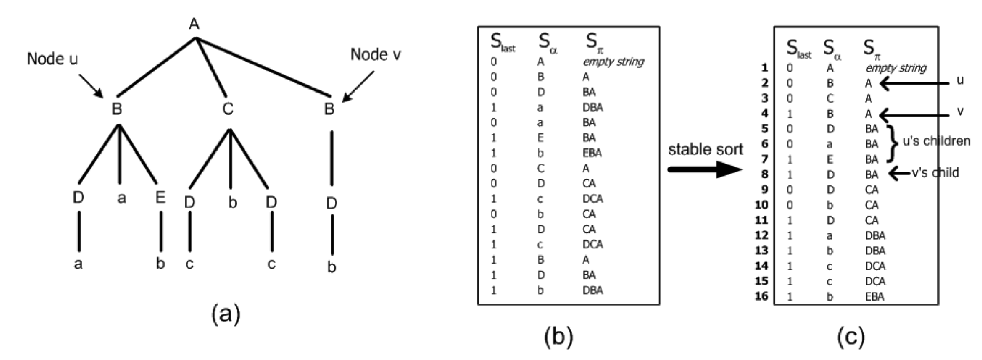
\includegraphics[width=1\textwidth]{Immagini/XBWT_example.png}
    \caption[XBWT example]{(a) A labeled tree $T$ where $\Sigma_N = \{A, B, C, D, E\}$ and $\Sigma_L = \{a, b, c\}$. Notice that $\alpha[u] = \alpha[v] = B$ and $\pi[u] = \pi[v] = A$. (b) The multi-set $S$ is obtained after the pre-order visit of $T$. (c) The final multi-set $S$ after the stable sort based on the $\pi$'s component of its triplets.}
    \label{fig:XBWT_example}
\end{figure}
\end{comment}

\subsubsection{Skew Algorithm}
The Skew algorithm is an efficient method for constructing the suffix array of a string in linear time. A suffix array is a data structure that lists the starting indices of all the suffixes of a string in lexicographical order, and it is widely used in various string processing algorithms.

\subsubsection*{Algorithm Overview}

\subsubsection*{1. Divide the String}

The algorithm begins by partitioning the indices of the string into three groups based on their modulo 3 value:
\begin{itemize}
    \item $S_0$: Indices congruent to 0 mod 3.
    \item $S_1$: Indices congruent to 1 mod 3.
    \item $S_2$: Indices congruent to 2 mod 3.
\end{itemize}

The suffixes starting at positions in $S_1$ and $S_2$ are combined into a single group called $S_{12}$.

\subsubsection*{2. Sort Suffixes in $S_{12}$}

To sort the suffixes in $S_{12}$, the algorithm considers the triplets of characters starting at each position in $S_{12}$. These triplets are sorted using a linear-time sorting algorithm, such as radix sort, and then renamed by assigning each triplet an integer value representing its rank in the sorted order. If all triplets are unique, the sorting is complete; otherwise, the same procedure is applied recursively to the sequence of ranks obtained.

\subsubsection*{3. Sort Suffixes in $S_0$}

Once the suffixes in $S_{12}$ are sorted, the algorithm proceeds to sort the suffixes in $S_0$. To compare two suffixes starting at positions $i$ and $j$ in $S_0$, it compares the first characters of their respective substrings. If the characters are different, their lexicographical order is immediately determined. If they are equal, the algorithm compares the suffixes starting at positions $i+1$ and $j+1$, whose ranks are already known from the sorting of $S_{12}$.

\subsubsection*{4. Merge the Sorted Orders}

Finally, the sorted orders of the suffixes in $S_0$ and $S_{12}$ are merged to obtain the complete suffix array of the original string. This merging process can be performed in linear time, ensuring the overall efficiency of the algorithm.

\subsubsection{PathSort Algorithm} \label{sec:pathSort}

The pseudocode of the pathSort algorithm is shown in \cref{alg:pathSort}. As we can see, the algorithm is based on the Skew algorithm, but it is adapted to work on labeled trees. 
Given a value $j\in\{0,1,2\}$, the main idea is to recursively sort the upward subpaths of the tree starting at nodes in levels $\not\equiv j \pmod{3}$, then sort the upward subpaths starting at nodes in levels $\equiv j \pmod{3}$ using the result of the previous step, and finally merge the two sets of sorted subpaths by exploiting their lexicographic names. $j$ is chosen in such a way that the number of nodes of the shrunk tree whose level is $\equiv j \pmod{3}$ is at least $t/3$ so that a constant fraction of upward paths are ensured to be dropped at each recursive step.
Is important to note that:
\begin{enumerate}
    \item the height of the new (contracted) tree shrinks by a factor of three, hence the node naming requires the radix sort over triples of names; 
    \item given the choice of $j$, the number of nodes of the new (contracted) tree will be at most $2t/3$, thus ensuring that the running time of the algorithm satisfies the recurrence $R(t) = R(2t/3) + \Theta(t) = \Theta(t)$; 
    \item following an argument similar to \cite{karkkainen2006linear}, the names of the dropped subpaths can be computed in $O(t)$ time from the names of the non-dropped subpaths, by radix sorting.
\end{enumerate}

\begin{algorithm}
    \caption{\textsc{PathSort}($T$)}
    \label{alg:pathSort}
    \begin{algorithmic}[1]
    \State Create the array \texttt{IntNodes}[1, $t$], initially empty.
    \State Visit the internal nodes of $T$ in pre-order. Let $u$ denote the $i$-th visited node.
    \State Write in \texttt{IntNodes}[$i$] the symbol $\alpha(u)$, the level of $u$ in $T$, and the position in \texttt{IntNodes} of $u$'s parent.
    \State Let $j \in \{0, 1, 2\}$ be such that the number of nodes in \texttt{IntNodes} whose level is $\equiv j \pmod{3}$ is at least $t/3$. Sort recursively the upward subpaths starting at nodes in levels $\not\equiv j \pmod{3}$.
    \State Sort the upward subpaths starting at nodes in levels $\equiv j \pmod{3}$ using the result of Step 3.
    \State Merge the two sets of sorted subpaths by exploiting their lexicographic names.
    \end{algorithmic}
\end{algorithm}

\subsubsection{Recursive Step of PathSort}
At each recursive step, the algorithm constructs the array \texttt{IntNodes}, which stores the triplets $(\alpha(u), \text{level}(u), \text{parent}(u))$ for every internal node $u$ in the given tree $T$.  

Next, the algorithm selects a value $j$ such that the number of nodes in \texttt{IntNodes} with depth $\equiv j \pmod{3}$ is at least $t/3$. Based on this choice, two separate arrays are created:  
\begin{itemize}
    \item \texttt{IntNodesAtPosJ}, containing nodes at levels $\equiv j \pmod{3}$,
    \item \texttt{IntNodesNotAtPosJ}, containing nodes at levels $\not\equiv j \pmod{3}$
\end{itemize}

For each node $u$ in \texttt{IntNodesNotAtPosJ}, the algorithm extracts the upward path consisting of the first three ancestors of $u$. These paths are then sorted using radix sort. If the sorted upward paths contain duplicates, the algorithm recursively calls the PathSort function on a new contracted tree, where nodes are renamed according to their sorted paths. Otherwise, if all upward paths are unique, the nodes in \texttt{IntNodesAtPosJ} are sorted and subsequently merged with \texttt{IntNodesNotAtPosJ} using lexicographic ordering, following the same merging strategy as in the Skew algorithm.

\subsection{Inversion}
The ability to invert the XBWT is fundamental to its utility as a compression technique. Invertibility guarantees that the original tree can be perfectly reconstructed from its transformed representation ($S_{\text{last}}$ and $S_{\alpha}$). This ensures that the compression is lossless, meaning no information is lost during the process, which is a critical requirement for most applications.

Property 'Path-based Indexing' (\cref{prop3}) ensures that the two arrays $S_{\text{last}}$ and $S_{\alpha}$ of the XBWT can be used to reconstruct the original tree $T$. The algorithm to invert the XBWT is linear in time and requires $O(t \log t)$ bits of space.

\cref{alg:rebuildTree} operates in three main steps. First, it constructs two auxiliary arrays, $F$ and $J$, which are crucial for navigating the tree structure within the compressed format.

\begin{itemize}
    \item \textbf{The $F$ array:} This array maps each character $c \in \Sigma$ to the index of the first occurrence in $S$ of a triplet whose $\pi$-component is prefixed by $c$. It essentially marks the starting points of blocks of nodes that share the same initial path label.
    \item \textbf{The $J$ array:} For each entry $i$ in $S$, $J[i]$ stores the index in $S$ corresponding to the first child of the node represented by $S[i]$. If $S[i]$ represents a leaf, $J[i]$ is set to a sentinel value (e.g., -1).
\end{itemize}

\begin{example}[$F$ and $J$ arrays]
    Considering the XBWT in \cref{tab:xbwt_example}, the $F$ array would map 'A' to index 2 (for node $r$), 'B' to index 5 (for the children of nodes with label 'B'), and so on. For the $J$ array, let's take the node $u$ at index 2 in $S$. Its first child is at index 5. Therefore, $J[2]$ would be 5.
\end{example}

Finally, the algorithm employs the array $J$ to
simulate a depth-first visit of $T$, creates its labeled nodes, and properly connects them to their parents. 

\begin{algorithm}[H]
    \caption{RebuildTree(\texttt{XBWT[$T$]})}
    \label{alg:rebuildTree}
    \begin{algorithmic}[1]
    \State $F = $ BuildF(\texttt{XBWT[$T$]});
    \State $J = $ BuildJ(\texttt{XBWT[$T$]}, $F$); 
    \State Create node $r$ and set $Q = \{\langle1, r\rangle\}$; \Comment{$Q$ is a stack}
    \While{$Q \neq \emptyset$} \Comment{We still have nodes to create in $T$}
        \State $\langle i, u \rangle = $ pop($Q$);
        \State $j = J[i]$; \Comment{Take the block of $u$'s children in $S$}
        \If{$j = -1$} \Comment{$u$ is a leaf of $T$}
            \State \textbf{continue};
        \EndIf
        \State Find first $j' \geq j$ such that $S_{\text{last}}[j'] = 1$; \Comment{$S[j, j']$ are the children of $u$ in $T$}
        \For{$h = j'$ downto $j$} \Comment{Recall that $Q$ is a stack}
            \State Create the node $v$ labeled $S_\alpha[h]$;
            \State Attach $v$ as first child of $u$;
            \State push($\langle h, v \rangle$, $Q$);
        \EndFor
    \EndWhile
    \State \Return node $r$.
    \end{algorithmic}
\end{algorithm}

\begin{algorithm}[H]
    \caption{BuildF(\texttt{XBWT[$T$]})}
    \label{alg:buildF}
    \begin{algorithmic}[1]
    \For{$i = 1, \ldots, |\Sigma_N|$}
        \State $C[S_\alpha[i]] \gets C[S_\alpha[i]] + 1$; \Comment{Count the occurrences of node labels}
    \EndFor
    \State $F[1] = 2$; \Comment{$S_\pi[1]$ is the empty string}
    \For{$i \in \{1, \ldots, |\Sigma_N|-1\}$} \Comment{Consider just the internal-node labels}
        \State $s = 0$; $j = F[i]$;
        \While{$s \neq C[i]$} \Comment{Not all blocks of children have been passed}
            \State $j = j + 1$;
            \If{$S_{\text{last}}[j] = 1$} \Comment{One further block of children has passed}
                \State $s = s + 1$;
            \EndIf
        \EndWhile
        \State $F[i+1] = j$;
    \EndFor
    \State \Return $F$.
    \end{algorithmic}
\end{algorithm}
    
\begin{algorithm}[H]
    \caption{BuildJ(\texttt{XBWT[$T$]}, $F$)}
    \begin{algorithmic}[1]
    \For{$i = 1, \ldots, t$}
        \If{$S_\alpha[i] \in \Sigma_L$}
            \State $J[i] = -1$; \Comment{$S_\alpha[i]$ is a leaf label}
        \Else
            \State $z = J[S_\alpha[i]]$;
            \While{$S_{\text{last}}[z] \neq 1$} \Comment{Reach the last child of $S_\alpha[i]$}
                \State $z = z + 1$;
            \EndWhile
            \State $F[S_\alpha[i]] = z + 1$;
        \EndIf
    \EndFor
    \State \Return $J$.
    \end{algorithmic}
\end{algorithm}

\subsection{Compressing Labeled Trees}
\begin{comment}
Let the $k$-context of a node $u \in T$ be the first $k$ symbols of $\pi(u)$. We denote this $k$-long prefix as $\pi_k[u]$. Thus, $\pi_k[u]$ represents the subpath of length $k$ leading to $u$ in $T$, or equivalently, the node $u$ descends from a subpath labeled as $\pi_k[u]$, where the nodes in $\pi_k[u]$ are encountered in an upward direction.
\end{comment}

The XBWT[$T$] exhibits a local homogeneity property on the string $S_{\alpha}$, specifically, node labels get distributed over $S_{\alpha}$ in accordance with a pattern that clusters closely the labels that descend from `similar' upward paths sharing long prefixes. Which can be demonstrated through the concept of $k$-contexts on trees. 
This property mirrors the strong local homogeneity exhibited by strings under the Burrows-Wheeler Transform \cite{burrows1994block} when applied to labeled trees.

To illustrate this, let us consider two arbitrary nodes $u$ and $v$ in $T$, and examine their contexts $\pi(u)$ and $\pi(v)$. Given the sorting of $S$, the greater the length of the shared prefix between $\pi(u)$ and $\pi(v)$, the closer the corresponding labels $\alpha(u)$ and $\alpha(v)$ will be in the string $S_{\alpha}$. These closely spaced labels are expected to be few in number, resulting in $S_{\alpha}$ exhibiting local homogeneity. As a consequence, we can leverage the advanced algorithmic techniques developed for BWT-based compression methods to achieve efficient compression.

At the end, the XBWT is used for turning the labeled tree compression problem into a string compression problem. To this aim, two string compressors
$C_{\alpha}$ and $C_{\text{last}}$ are used to compress the two strings that compose XBWT[$T$], by exploiting their fine specialties. Of course, many choices are possible for $C_{\alpha}$ and $C_{\text{last}}$, each having implications on the algorithmic time and compression bounds.

In general, the following theorem holds:

\begin{theorem}
    let $C_{\alpha}$ be a $k$-th order string compressor that compresses any string $w$ into $|w|H_k(w) + |w| + o(|w|)$ bits, taking $O(|w|)$ time; and let $C_{\text{last}}$ be an algorithm that stores $S_{\text{last}}$ without compression. With this simple instantiation, the labeled tree $T$ can be compressed within $t H_k(S_{\alpha}) + 2t + o(t)$ bits and takes $O(t)$ optimal time.
\end{theorem}

Since $H_k(S_\alpha) \leq (\log |\Sigma|) + 1,^6$ the above bound is at most $t(\log |\Sigma| + 3) + o(t)$ bits, and can be significantly better than the information-theoretic lower bound and the plain storage of XBWT[$T$] (both taking $2t + t \log|\Sigma|$ bits), depending on the distribution of the labels among its nodes.

\subsection{Indexing a Compressed Labeled Tree} \label{sec:xbwt_operations}
In order to implement the efficient operations listed in \cref{compandindexinglabtree} using the compressed arrays $S_{\text{last}}$ and $S_{\alpha}$ of XBWT, we need that the chosen compressors $C_{\alpha}$ and $C_{\text{last}}$ support the following operations:

Given a string $S[1, t]$ over alphabet $\Sigma$
\begin{itemize}
    \item \textbf{$rank_c(S, q)$}: gives the number of times the symbol $c \in \Sigma$ appears in $S[1, q]$.
    \item \textbf{$select_c(S, i)$}: gives the position of the $i$-th occurrence of the symbol $c \in \Sigma$ in $S$.
\end{itemize}

The compressed indexing of XBWT[$T$] will be based on three compressed data structures that support rank and select queries over the two strings $S_{\alpha}$ and $S_{\text{last}}$, and over an auxiliary binary array $A[1, t]$ defined as: $A[1] = 0$, $A[j] = 1$ if and only if the first symbol of $S_{\pi}[j]$ differs from the first symbol of $S_{\pi}[j - 1]$. 
Hence, $A$ contains at most $|\Sigma| + 1$ bits set to 1 out of $t$ positions. It is also easy to see that, through rank and select operations over $A$, we can succinctly implement the array $F$ employed in \cref{alg:rebuildTree,alg:buildF}.

The following methods are supported by the compressed index:

\textbf{GetRankedChild(i, k)}: Returns the position in $S$ of the $k$-th child of the node at index $i$. If the child does not exist, it returns -1. 
\begin{example}
    In \cref{tab:xbwt_example}, \texttt{GetRankedChild(2, 2)} returns 6.
\end{example}

\textbf{GetCharRankedChild(i, c, k)}: Returns the position in $S$ of the $k$-th child labeled $c$ of the node at index $i$. If the child does not exist, it returns -1.
\begin{example}
    In \cref{tab:xbwt_example}, \texttt{GetCharRankedChild(1, B, 2)} returns 4.
\end{example}

\textbf{GetDegree(i)}: Returns the total number of children of the node at index $i$ in $S$.

\textbf{GetCharDegree(i, c)}: Returns the number of children of the node at index $i$ in $S$ that have the label $c$.

\textbf{GetParent(i)}: Returns the position in $S$ of the parent of the node at index $i$. If the node is the root (at index 1), it returns -1.
\begin{example}
    In \cref{tab:xbwt_example}, \texttt{GetParent(8)} returns 4.
\end{example}

\textbf{GetSubtree(i)}: Retrieves the labels of all nodes in the subtree rooted at the node at index $i$ in $S$. The labels can be returned in any standard traversal order (e.g., pre-order, in-order, or post-order).

\textbf{SubPathSearch($P$)}: For a given labeled path $P = c_1c_2 \cdots c_k$, this function finds the range $S[\text{First} \dots \text{Last}]$ containing the immediate children of all nodes that match the path $P$. Meaning that all strings in $S_{\pi}[\text{First} \dots \text{Last}]$ are prefixed by the reversed path $P^R = c_k \cdots c_2c_1$, as the strings in $S_{\pi}$ are constructed using upward paths.
\begin{example}
    In \cref{tab:xbwt_example}, \texttt{SubPathSearch(BD)} results in the range [12, 13], and \\ \texttt{SubPathSearch(AB)} gives the range [5, 8].
\end{example}

It is important to note that their time complexity is dependent on the specific implementation for rank and select over the compressed strings $S_{\alpha}$ and $S_{\text{last}}$. 

Let's now see how to implement some of the above methods (from which the others can be derived) using the rank and select operations over the compressed strings $S_{\alpha}$ and $S_{\text{last}}$.

\begin{table}
    \centering
    \begin{tabular}{r c c c l}
    \hline\hline
    \textbf{} & $A$ & \textbf{$S_{\text{last}}$} & \textbf{$S_{\alpha}$} & \textbf{$S_{\pi}$} \\
    \hline
    \textbf{1} & 0 & 0 & A & \textit{empty string} \\
    \textbf{2} & 1 & 0 & B & A \\
    \textbf{3} & 0 & 0 & C & A \\
    \textbf{4} & 0 & 1 & B & A \\
    \textbf{5} & 1 & 0 & D & BA \\
    \textbf{6} & 0 & 0 & a & BA \\
    \textbf{7} & 0 & 1 & E & BA \\
    \textbf{8} & 0 & 1 & D & BA \\
    \textbf{9} & 1 & 0 & D & CA \\
    \textbf{10} & 0 & 0 & b & CA \\
    \textbf{11} & 0 & 1 & D & CA \\
    \textbf{12} & 1 & 1 & a & DBA \\
    \textbf{13} & 0 & 1 & b & DBA \\
    \textbf{14} & 0 & 1 & c & DCA \\
    \textbf{15} & 0 & 1 & c & DCA \\
    \textbf{16} & 1 & 1 & b & EBA \\
    \hline\hline
    \end{tabular}
    \caption{The multi-set $S$ for the tree shown in \cref{fig:example_tree}, obtained by stably sorting triplets according to their '$\pi$' components. In this representation, nodes $u$ and $v$ from the original tree $T$ appear at indices $2$ and $4$, respectively. The children's block of node $u$ occupies positions $5$ through $7$, while node $v$'s single child is located at index $8$. Also, the auxiliary binary array $A$ is shown.}
    \label{tab:xbwt_example_2}
\end{table}

\subsubsection*{GetChildren(i)}
\cref{alg:getchildren} exploits directly the properties described before, in particular Property `Path-based Indexing' (\cref{prop3}). The rank operation at line 5 is used to get the number $r$ of nodes labeled $c$ up to position $i$ in $S_{\alpha}$. Then, the position $F[c]$ is obtained through a select operation on $A$ (line 6). By Property `Path-based Indexing', the children of $S[i]$ are located at the $r$-th block of children following position $F[c]$. Lines $8 - 9$ identify this block. 

\begin{example}
    Let's walk through an example using \cref{tab:xbwt_example_2}. Consider the node $u$ at index 2 labeled with $B$. To find its children:

    \begin{enumerate}
        \item First, we compute $r = 1$ since this is the first occurrence of $B$ in $S_{\alpha}$ up to position 2.
        \item Next, we find $y = F[B] = 5$, which marks the start of the block containing children of all nodes labeled $B$.
        \item Then, we count $z = 1$ ones in $S_{\text{last}}$ up to position $y-1$.
        \item Finally, the children block is delimited by the $z+r-1 = 1$st and $z+r = 2$nd ones in $S_{\text{last}}$, giving us the range $[5,7]$.
    \end{enumerate}

    This range $[5,7]$ indeed contains the three children of the node at index 2, as we can verify from the tree structure in \cref{fig:example_tree}.
\end{example}

\begin{algorithm}[H] 
    \caption{GetChildren($i$)}
    \label{alg:getchildren}
    \begin{algorithmic}[1]
    \If{$S_\alpha[i] \in \Sigma_L$}
        \State \Return $-1$ \Comment{$S[i]$ is a leaf}
    \EndIf
    \State $c \gets S_\alpha[i]$ \Comment{$S[i]$ is labeled $c$}
    \State $r \gets \text{rank}_c(S_\alpha, i)$
    \State $y \gets \text{select}_1(A, c)$ \Comment{$y = F[c]$}
    \State $z \gets \text{rank}_1(S_{\text{last}}, y - 1)$
    \State $\text{First} \gets \text{select}_1(S_{\text{last}}, z + r - 1) + 1$
    \State $\text{Last} \gets \text{select}_1(S_{\text{last}}, z + r)$
    \State \Return $(\text{First}, \text{Last})$
    \end{algorithmic}
\end{algorithm}

\subsubsection*{GetParent(i)}
\cref{alg:getparent} is based on Property `Path-based Indexing' (\cref{prop3}) and it is the inverse of the GetChildren method. In line 4, the algorithm computes the label $c$ of the parent of $S[i]$ that prefixes the upward path leading to $S[i]$. Then, the parent of $S[i]$ is searched among the nodes labeled $c$ in $S_{\alpha}$ by exploiting Property `Path-based Indexing' in a reverse manner. Namely, the number $k$ of children-blocks in the range $S[y, i]$ is computed; these are children of nodes labeled $c$ and preceding $i$ in the stable sort of $S$. Then, the $k$-th occurrence of $c$ in $S_{\alpha}$ is selected, which is indeed the parent of $S[i]$.

\begin{example}
    Let's illustrate how to find a node's parent using \cref{tab:xbwt_example_2}. Consider node $v$ located at index 4 with label $B$. The process to find its parent involves:
    \begin{enumerate}
        \item Computing $c = \text{rank}_1(A, 4) = 1$, which tells us the parent has label `A' (as $A$ contains exactly one 1 up to position 4).
        \item Locating $y = F[A] = 2$, which indicates where the block of children for nodes labeled `A' begins.
        \item Calculating $k = \text{rank}_1(S_{\text{last}}, 4-1) - \text{rank}_1(S_{\text{last}}, 2-1) = 0$, meaning no complete child blocks appear before position 4.
        \item Therefore, $v$'s parent is the first ($(k+1)$-th) occurrence of `A' in $S_{\alpha}$, corresponding to index 1 (the root of $\mathcal{T}$).
    \end{enumerate}
    This example demonstrates how the XBWT structure efficiently encodes parent-child relationships using just the $S_{\text{last}}$ and $S_{\alpha}$ arrays.
\end{example}

\begin{algorithm}[H]
    \caption{GetParent($i$)}
    \label{alg:getparent}
    \begin{algorithmic}[1]
    \If{$i = 1$}
        \State \Return $-1$ \Comment{$S[i]$ is the root of $\mathcal{T}$}
    \EndIf
    \State $c \gets \text{rank}_1(A, i)$
    \State $y \gets \text{select}_1(A, c)$
    \State $k \gets \text{rank}_1(S_{\text{last}}, i - 1) - \text{rank}_1(S_{\text{last}}, y - 1)$
    \State $p \gets \text{select}_c(S_\alpha, k + 1)$
    \State \Return $p$
    \end{algorithmic}
\end{algorithm}

\subsubsection*{SubPathSearch($P$)}
We assume that $P = c_1c_2 \cdots c_k$ algorithm SubPathSearch computes the range $[First, Last]$ in $|P| = l$ phases, each one preserving the following invariant:

\begin{itemize}
    \item Invariant of Phase $i$. At the end of the phase, $S_{\pi}[First]$ is the first entry prefixed by $P[1, i]^R$ , and $S_{\pi}[Last]$ is the last entry prefixed by $P[1, i]^R$ , where $s^R$ is the reversal of string $s$.
\end{itemize}

At the beginning (i.e., $i = 1$), First and Last are easily determined via the entries $F[c_1]$ and $F[c_1 + 1] - 1$, which point to the first and last entry of $S_{\pi}$ prefixed by $c_1$ (by definition of array $F$). Since we do not have the $F$ array, we implement these operations via rank and select queries over array $A$. Let us assume that the invariant holds for Phase $i - 1$, and prove that the $i$-th iteration of the for-loop in algorithm SubPathSearch preserves the invariant. More precisely, let $S_{\pi}[First, Last]$ be all entries prefixed by $P[1, i - 1]^R$. So $S[First, Last]$ contains all nodes descending from $P[1, i - 1]$. SubPathSearch determines $S[z_1]$ (respectively $S[z_2]$) as the first (respectively last) node in $S[First, Last]$ that descends from $P[1, i - 1]$ and is labeled $c_i$, if any. Then it jumps to the first child of $S[z_1]$ and the last child of $S[z_2]$. From Property 2 (item 2) and the correctness of algorithms GetChildren and GetDegree, we infer that the positions of these two children are exactly the first (respectively last) entry in $S$ whose $\pi$-component is prefixed by $P[1, i]^R$. 

The time complexity of the SubPathSearch algorithm is $O(l)$, where $l$ is the length of the input path $P$.

\begin{example}
    Consider the tree in \cref{fig:example_tree}, and let $P = BD$. The algorithm \textsc{SubPathSearch}($P$) returns the range $[12, 13]$ through the following steps:

    \begin{enumerate}
        \item Initially, $First = F[B] = 5$ and $Last = F[C] - 1 = 8$. The range $S[5,8]$ contains all nodes descending from paths prefixed by $B$.
        
        \item For $c_2 = D$:
        \begin{itemize}
            \item Compute $k_1 = 0$ and $k_2 = 2$
            \item This yields $z_1 = 5$ and $z_2 = 8$
            \item The first child of $S[5]$ is at position $12$
            \item The last (and only) child of $S[8]$ is at position $13$
        \end{itemize}
        
        \item Therefore, the algorithm returns the range $[12,13]$
    \end{enumerate}

    Note that both the number of offspring and the number of occurrences of subpath $P$ are 2, as evidenced by the two occurrences of 1 in $S_{\text{last}}[12,13]$.
\end{example}

\begin{algorithm}[H]
    \caption{SubPathSearch($P$)}
    \label{alg:subpathsearch}
    \begin{algorithmic}[1]
    \State $First \gets F(c_1)$; $Last \gets F(c_1 + 1) - 1$
    \If{$First > Last$}
        \State \textbf{return} ``$P$ is not a subpath of $T$''
    \EndIf
    \For{$i \gets 2, \dots, k$}
        \State $k_1 \gets \text{rank}_{c_i}(S_\alpha, First - 1)$; $z_1 \gets \text{select}_{c_i}(S_\alpha, k_1 + 1)$
        \Comment{first entry in $S_\alpha[First, t]$ labeled $c_i$}
        \State $k_2 \gets \text{rank}_{c_i}(S_\alpha, Last)$; $z_2 \gets \text{select}_{c_i}(S_\alpha, k_2)$
        \Comment{last entry in $S_\alpha[1, Last]$ labeled $c_i$}
        \If{$z_1 > z_2$}
            \State \textbf{return} ``$P$ is not a subpath of $T$''
        \EndIf
        \State $First \gets \text{GetRankedChild}(z_1, 1)$ \Comment{get the first child of $S[z_1]$}
        \State $Last \gets \text{GetRankedChild}(z_2, \text{GetDegree}(z_2))$ \Comment{get the last child of $S[z_2]$}
    \EndFor
    \State \textbf{return} $(First, Last)$
    \end{algorithmic}
\end{algorithm}

\section{Implementation}
The XBWT data structure has been implemented in C++ using the Succinct Data Structure Library 2.0 (SDSL) for efficient representation and manipulation of compressed data structures. We will develop two algorithms for constructing the XBWT: one efficient linear-time recursive algorithm and one more straightforward iterative algorithm. Also, we will implement the necessary data structures and algorithms for navigating and querying the XBWT, such as parent-child navigation and path-based searches. 

The implementation of the XBWT is based on the descriptions provided in the previous sections. Also, it is available on GitHub at the following link: \url{https://github.com/davide-tonetto-884585/XBWT}.

\subsection{Implementation Choices}
Follows a list of the main choices made during the implementation of the XBWT:
\begin{itemize}
    \item The implementation is not focused on a specific kind of data, such as XML documents or JSON files, but it is designed to work with any kind of labeled tree. 
    \item The construction method takes as input a labeled tree. It constructs directly a compressed indexing scheme based on the Extended Burrows-Wheeler Transform of the tree as described in the previous sections.
    \item For the XBWT to work, we assume that the labels of the leaf nodes of the given labeled tree are lexicographically greater than the labels of the internal nodes. This is necessary to ensure that the navigational and search operations work correctly. \draft{This can be obtained by...} \alessio{spiega come si ottiene questo risultato nel caso le foglie siano più piccole.}
    \item The implementation is based on the Succinct Data Structure Library (SDSL) to handle the compressed data structures generated by the XBWT. The SDSL library provides efficient implementations of various compressed data structures and algorithms, which are essential for representing and querying the XBWT efficiently.
    \item The labels of the alphabet are encoded as integers, starting from 0 to $|\Sigma| - 1$, where $|\Sigma|$ is the cardinality of the alphabet. This encoding respects the order of the labels in the alphabet and allows simplifying and reducing the space needed to store the labels in the compressed data structure. For this reason, the constructor of the XBWT class takes as input a generic labeled tree.
    \item All the operations introduced in \cref{sec:xbwt_operations} are implemented in the XBWT class.
\end{itemize}

\subsection{Succinct Data Structures}
The implementation of the XBWT relies heavily on succinct data structures to achieve space efficiency while maintaining fast query operations. In particular, we use succinct data structures to compress the two main arrays of the XBWT: $S_\alpha$ and $S_{\text{last}}$. These arrays, which can be quite large for substantial trees, benefit significantly from compression.

The compression is achieved through the Succinct Data Structure Library (SDSL), which provides efficient implementations of various compressed data structures. For $S_{\text{last}}$, which is a binary sequence, we utilize a compressed bit vector that supports fast rank and select operations. For $S_\alpha$, which contains labels from a potentially large alphabet, we employ a wavelet tree structure that provides both compression and efficient query capabilities.

The SDSL is a C++ library that provides efficient implementations of various compressed data structures and algorithms. It is used in this project to handle the compressed data structures generated by the XBWT. The SDSL library provides a wide range of succinct data structures, such as bit vectors, wavelet trees, and compressed suffix arrays, which are essential for representing and querying the XBWT efficiently. The library is available at \url{https://github.com/simongog/sdsl-lite} \cite{gbmp2014sea}. Let's see the implementation details of the SDSL data structures used in the XBWT implementation.

\subsubsection{RRR Bit Vector}
The RRR bit vector is designed to provide space-efficient representations of bit vectors while supporting efficient rank and select operations. This data structure implements the RRR (Raman, Raman, and Rao) encoding method, which compresses bit vectors by partitioning them into fixed-size blocks and encoding each block based on its population count (the number of 1s) and specific configuration \cite{raman2002succinct}. 

The space needed for an RRR bit vector of length $n$ with $m$ set bits is $nH_0 + o(n)$ ($\approx \lceil \log \binom{n}{m} \rceil$). 
The rank support is provided by \texttt{sdsl::rank\_support\_rrr}, adding $80$ bits and requiring $O(\log k)$ time for rank queries, where $k$ is the number of set bits. The select support is provided by \texttt{sdsl::select\_support\_rrr}, adding $64$ bits and requiring $O(\log n)$ time for select queries.

This data structure is used to represent the $S_{\text{last}}$, the additional bit in $S_{\alpha}$, and $A$ arrays of the XBWT.

\subsubsection{Wavelet Tree}
The Wavelet tree is designed to efficiently handle sequences over large alphabets, such as integer sequences. It provides a space-efficient representation while supporting fast access, rank, and select operations. The wavelet tree is a balanced binary tree that recursively partitions the alphabet into two equal-sized subsets and encodes the sequence based on the partitioning \cite{grossi2003high}. The \texttt{sdsl::wt\_int} uses the RRR bit vectors or other succinct representations for storing the bit vectors in each node of the wavelet tree. This makes the structure space-efficient.

In the case of RRR bit vectors the space needed by integer Wavelet tree for a sequence of length $n$ over an alphabet of size $\sigma$ is $nH_0(S) + o(n \log \sigma) + \Theta(\sigma \log n)$ bits, where $H_0(S)$ is the zero-order empirical entropy of the sequence $S$. Also supports query access, rank, and select operations in $O(\log \sigma)$ time.

This data structure is used to represent the $S_\alpha$ array of the XBWT.

\begin{comment}
\subsection{Details of the XBWT Class Elements}
\alessio{Questa sezione non mi convince. Non descrivere troppo il codice, la documentazione dovrebbe essere nella repo e nel codice, non nella tesi.}
The XBWT class utilizes several data structures from the SDSL library to efficiently represent and query the compressed data. Below are the details of the main elements used in the class:

\begin{itemize}
    \item \texttt{sdsl::rrr\_vector<> SLastCompressed}: This is a compressed bit vector that stores the $S_{\text{last}}$ array of the XBWT. 
    \item \texttt{sdsl::wt\_int<sdsl::rrr\_vector<>> SAlphaCompressed}: This is a wavelet tree built on top of a compressed bit vector. The wavelet tree is used to compress and index the $S_{\alpha}$ array of the XBWT.
    \item \texttt{sdsl::rrr\_vector<> SAlphaBitCompressed}: Another compressed bit vector used to store the additional bit of $S_{\alpha}$ needed to distinguish between internal and leaf nodes.
    \item \texttt{sdsl::rrr\_vector<> ACompressed}: A compressed bit vector representing the $A$ array of the XBWT used to in the $F$ array of the XBWT.
    \item \texttt{sdsl::rrr\_vector<>::rank\_1\_type SLastCompressedRank}: A rank support structure for the \texttt{SLastCompressed} bit vector, allowing efficient rank queries.
    \item \texttt{sdsl::rrr\_vector<>::select\_1\_type SLastCompressedSelect}: A select support structure for the \texttt{SLastCompressed} bit vector, allowing efficient select queries.
    \item \texttt{sdsl::rrr\_vector<>::rank\_1\_type ACompressedRank}: A rank support structure for the \texttt{ACompressed} bit vector.
    \item \texttt{sdsl::rrr\_vector<>::select\_1\_type ACompressedSelect}: A select support structure for the \texttt{ACompressed} bit vector.
    \item \texttt{std::unordered\_map<T, unsigned int> alphabetMap}: A hash map that maps each label in the alphabet to a unique integer.
    \item \texttt{unsigned int cardSigma}: The cardinality of the alphabet $\Sigma$.
    \item \texttt{unsigned int cardSigmaN}: The cardinality of the $\Sigma_N$ alphabet. Where $\Sigma_N$ is the set of labels that appear in the internal nodes of the labeled tree.
    \item \texttt{unsigned int maxNumDigits}: The maximum number of digits that has the integer code associated to the greater label in the alphabet (needed to sort the labels in the alphabet).
\end{itemize}

The overall space complexity of the XBWT class can be derived from the space complexity of the compressed data structures used in the class. 

\subsection{Construction implementation}
\alessio{Perché non fare pseudocodice come per Alg 1?}
The construction of the XBWT is done by the constructor of the XBWT class. The constructor takes as input a generic labeled tree and constructs the compressed indexing scheme using the linear pathSort (also the naive construction method can be used by passing the boolean flag \texttt{usePathSort = false}). The construction process is divided into the following steps:

\begin{enumerate}
    \item \textbf{Alphabet Encoding}: The first step is to encode the labels of the alphabet as integers. The labels are sorted in lexicographical order and assigned a unique integer code starting from 1 to $|\Sigma|$. Two hash maps are used to map each label to a unique integer and vice versa. 
    \item \textbf{Construct \texttt{intNodes} array}: The next step is to construct the \texttt{intNodes} array as described in the previous chapters. \texttt{intNodes} is an array of triplets of length $t$ in which node is represented as a triplet containing the node's label, its level, and the index of its parent node in the array (from 1 to t, root has parent 0). The nodes are inserted in preorder traversal of the labeled tree.
    \item \textbf{Sort \texttt{intNodes} array:} Call the \texttt{pathSort} or \texttt{upwardStableSortConstruction} (naive method) method to get the sorted array of nodes \texttt{intNodes}.
    \item \textbf{Construct $S_{\text{last}}$ array}: Construct the $S_{\text{last}}$ array by iterating over the sorted \texttt{intNodes} array.
    \item \textbf{Construct $S_{\alpha}$ array}: Construct the $S_{\alpha}$ array by iterating over the sorted \texttt{intNodes} array, along with the additional bit array to distinguish between internal and leaf nodes.
    \item \textbf{Construct $A$ array}: Construct the $A$ array by iterating over the sorted \texttt{intNodes} array.
    \item \textbf{Construct rank and select support structures}: Construct the rank and select support structures for the compressed bit vectors.
\end{enumerate}

\subsection{Navigational Operations}
\alessio{Non basta dire che implementi tutte le funzioni descritte nella sezione 3.7?}

The XBWT class provides several navigational operations to traverse the labeled tree and retrieve information about the nodes. The navigational operations implemented are:

\begin{itemize}
    \item \texttt{getChildren(unsigned int i)}: This method returns a pair of integers representing the indices of the leftmost and rightmost children of the node at index \texttt{i}.
    \item \texttt{getRankedChild(unsigned int i, unsigned int k)}: This method returns the index of the \texttt{k}-th child of the node at index \texttt{i}.
    \item \texttt{getCharRankedChild(unsigned int i, T label, unsigned int k) const}: This method returns the index of the \texttt{k}-th child of the node at index \texttt{i} with the specified label.
    \item \texttt{getDegree(unsigned int i)}: This method returns the degree (number of children) of the node at index \texttt{i}.
    \item \texttt{getCharDegree(unsigned int i, T label)}: This method returns the number of children of the node at index \texttt{i} with the specified label.
    \item \texttt{getParent(unsigned int i)}: This method returns the index of the parent of the node at index \texttt{i}.
    \item \texttt{getSubtree(unsigned int i, unsigned int order = 0)}: This method returns a vector containing the labels of the nodes in the subtree rooted at index \texttt{i}. The \texttt{order} parameter specifies the traversal order (e.g., preorder, post-order).
\end{itemize}

All the methods refer to the index of the nodes in $S_{\text{last}}$ and $S_{\alpha}$ arrays. 

\subsection{Search Operations}
The XBWT class provides search operation \texttt{subPathSearch(const std::vector<T> \&path)} that searches for a subpath in the XBWT structure. It uses the compressed vectors to determine the range of positions corresponding to the nodes whose upward path is prefixed by a given vector reversed.

\end{comment}

\subsection{Construction Time Experiments} 

To evaluate the performance of the implemented algorithms, we conducted a series of experiments on randomly generated trees, with sizes ranging from 100 to 900,000 nodes. For each tree, we executed the construction algorithms 10 times, recording the average execution time for both the linear \textsc{PathSort} algorithm and the Naive Sort algorithm used for constructing the XBWT.
By ``Naive Sort'', we refer to a straightforward approach that first precomputes all the upward paths in the tree and then sorts them using a standard sorting algorithm. This method contrasts with \textsc{PathSort}, which is specifically designed to achieve linear time complexity in path sorting.
This approach enabled us to compare their performance across various tree sizes and evaluate their scalability.

From the results shown in Table \cref{tab:experiments}, we can draw several conclusions about the performance of the \textsc{PathSort} algorithm compared to the Naive Sort algorithm.

The \textsc{PathSort} algorithm consistently outperforms the Naive Sort algorithm in terms of execution time, especially as the number of nodes increases. For smaller trees, the difference in execution time between the two algorithms is minimal. However, as the number of nodes grows, the \textsc{PathSort} algorithm demonstrates significantly better scalability. For instance, with 900,000 nodes, the \textsc{PathSort} algorithm takes 8.51 seconds, whereas the Naive Sort algorithm takes 34.2 seconds, giving a speedup of more than $4\times$. A visual representation of the results can be seen in \cref{fig:xbwt_exp_plots} where both the time comparison and the speedup are shown.

\begin{table}[h]
    \centering
    \begin{tabular}{|r|r||r|r|}
        \hline
        \textbf{\# Nodes} & \textbf{Depth} & \textbf{Naive Sort (s)} & \textbf{\textsc{PathSort} (s)} \\
        \hline
            100 &    22 &  0.001 & 0.002 \\
            500 &    45 &  0.002 & 0.004 \\
          1,000 &    74 &  0.003 & 0.006 \\
          5,000 &   175 &  0.015 & 0.028 \\
         10,000 &   288 &  0.053 & 0.056 \\
         50,000 &   486 &  0.350 & 0.310 \\
        100,000 &   754 &  1.250 & 0.690 \\
        500,000 & 2,246 & 16.460 & 4.700 \\
        900,000 & 2,658 & 34.200 & 8.510 \\
        \hline
    \end{tabular}
    \caption{Performance comparison of the execution times for the Naive Sort and \textsc{PathSort} algorithms on randomly generated trees of varying sizes.}
    \label{tab:experiments}
\end{table}

\begin{figure}[H]
    \centering
    \begin{subfigure}[b]{0.48\textwidth}
        \centering
        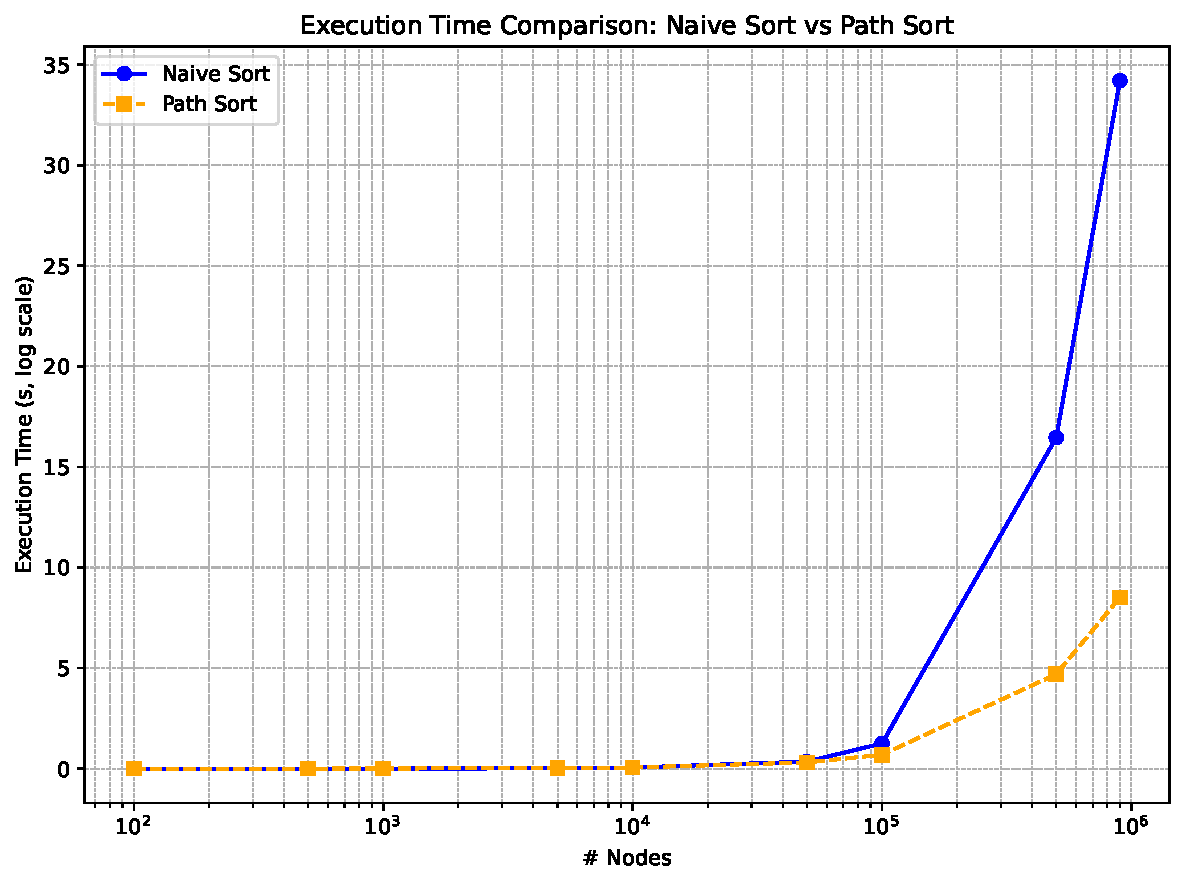
\includegraphics[width=\textwidth]{"Immagini/execution_time_comparison.pdf"}
        \caption{Time Comparison}
        \label{fig:time_comparison}
    \end{subfigure}
    \hfill %
    \begin{subfigure}[b]{0.48\textwidth}
        \centering
        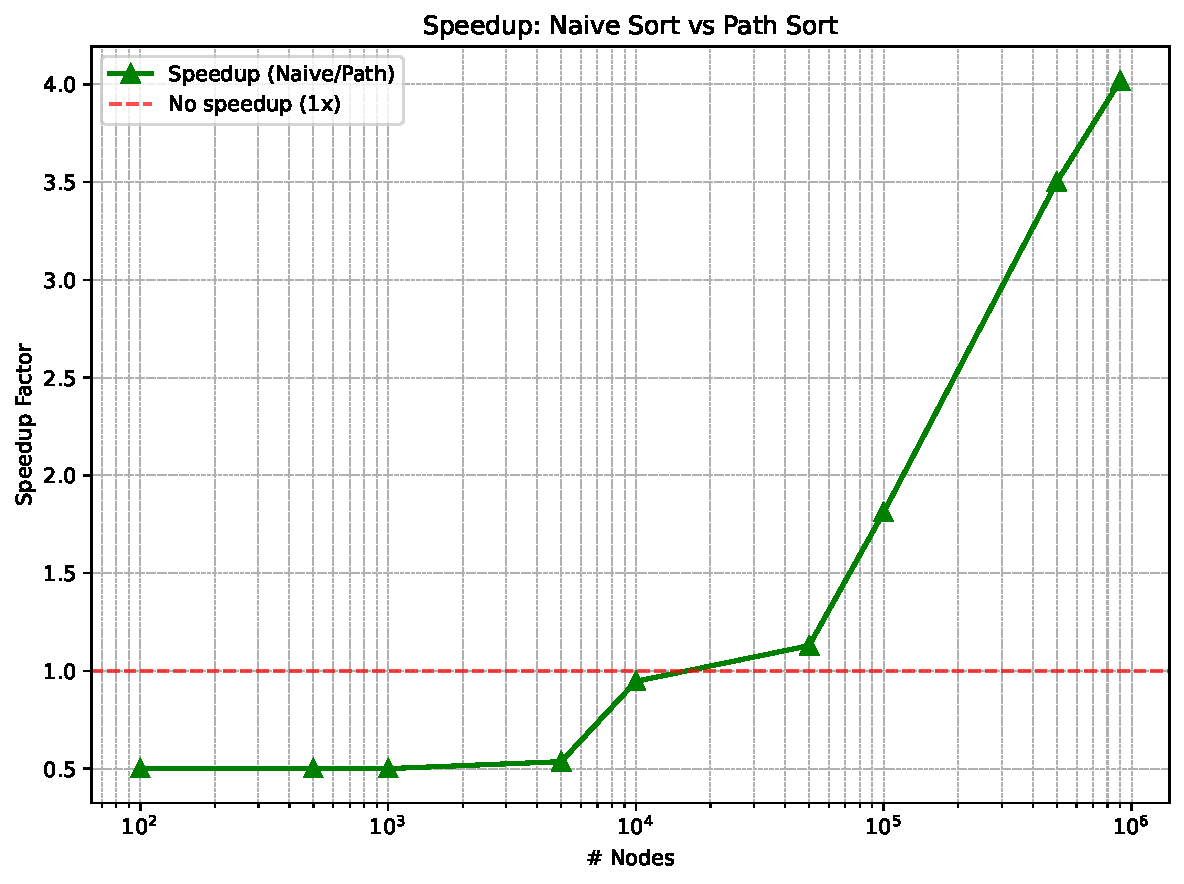
\includegraphics[width=\textwidth]{"Immagini/speedup_comparison.pdf"}
        \caption{Speedup}
        \label{fig:speedup}
    \end{subfigure}
    \caption{Time comparison and speedup plots for the experiments in \cref{tab:experiments}. Image (a) shows \textsc{PathSort} time in seconds (yellow dashed line) vs. Naive Sort time (blue line). Image (b) shows the speedup of \textsc{PathSort} over Naive Sort. The area below the red dashed line indicates points where the speedup is less than or equal to 1, representing no improvement of \textsc{PathSort} over Naive Sort.}
    \label{fig:xbwt_exp_plots}
\end{figure}

\begin{comment}
\subsubsection{Space Analysis}
To evaluate the space savings achieved through XBWT compression, we conducted experiments on the same set of randomly generated trees used for the construction performance tests. For each tree, we compared the memory usage (in bytes) of three representations: the plain tree, the uncompressed XBWT, and the compressed XBWT.

The plain tree representation consists of the simple balanced parentheses encoding of the tree structure combined with the edge labels. For example, for the tree in \cref{fig:example_tree,tab:xbwt_example}, the plain tree representation would be:

\texttt{(A(B(D(a))(a)(E(b)))(C(D(c))(b)(D(c)))(B(D(b))))}.

By \emph{uncompressed XBWT}, we refer to the XBWT arrays $S_{\text{last}}$ and $S_{\alpha}$ (including the additional bit) stored without any compression. Specifically, $S_{\text{last}}$ is represented as a plain bitvector (\texttt{sdsl::bit\_vector}), and $S_{\alpha}$ is stored as a wavelet tree (\texttt{sdsl::wt\_int}) with plain bitvectors (\texttt{sdsl::bit\_vector}). In contrast, the \emph{compressed XBWT} representation stores $S_{\text{last}}$ and $S_{A}$ as compressed RRR bitvectors (\texttt{sdsl::rrr\_vector}), and $S_{\alpha}$ as a wavelet tree with RRR bitvectors, as described in the previous chapter.

\cref{tab:experiments_2} reports the sizes (in bytes) for each representation of the trees across different sizes. The last column highlights the space savings achieved by the compressed XBWT compared to the plain tree representation, expressed as a percentage. These results illustrate the substantial space reductions achieved through compression, especially as the tree size increases.

%\alessio{Oltre ai punti di prima, metti la percentuale anche per UXBWT, magari non come un'altra colonna ma metti tra parentesi. Te lo faccio sulle prime righe per la C.XBWT. Se ti piace, ricorda di spiegare cosa sono i numeri tra parentesi nella descrizione.}
\begin{table}[ht]
    \centering
    \begin{tabular}{|r||r|r|r|}
        \hline
        \textbf{\# Nodes} & \textbf{Plain tree} & \textbf{U. XBWT} & \textbf{C. XBWT} \\
        \hline
            100 &       390 &       424 &       496 \color{gray}{(-27.18\%)}\\
            500 &     2,390 &     1,112 &     1,136 ~\color{gray}{(52.47\%)} \\
          1,000 &     4,890 &     2,242 &     2,056 ~\color{gray}{(57.96\%)} \\
          5,000 &    28,890 &    12,911 &    10,400 ~\color{gray}{(64.00\%)} \\
         10,000 &    58,890 &    45,625 &    21,848 ~\color{gray}{(62.90\%)} \\
         50,000 &   338,890 &   175,146 &   123,216 ~\color{gray}{(63.64\%)} \\
        100,000 &   688,890 &   349,478 &   259,376 ~\color{gray}{(62.35\%)} \\
        500,000 & 3,888,890 & 1,850,850 & 1,451,570 ~\color{gray}{(62.67\%)} \\
        900,000 & 7,088,890 & 3,480,190 & 2,718,570 ~\color{gray}{(61.65\%)} \\
        \hline
    \end{tabular}
    \caption{Space analysis of the XBWT. The first column represents the number of nodes, the others the bytes used by each representation.
    ``Plain tree'' is the size of the tree in the simple balanced parenthesis representation plus the edge labels, ``U. XBWT'' is the size of the uncompressed XBWT, and ``C. XBWT'' is the size of the compressed XBWT.
    Gray numbers between parentheses represent the improvement relative to the plain tree representation.}
    \label{tab:experiments_2}
\end{table}

For small trees, the compressed XBWT does not always provide immediate savings due to the overhead of succinct data structures. For instance, for 100 nodes, the compressed representation is larger than the plain tree, showing a \(-27.18\%\) increase in space. However, as the number of nodes increases, the compression becomes more effective, achieving savings of over 60\% for large trees.

The space reduction becomes particularly evident for trees with more than 500 nodes. These results confirm that the compressed XBWT provides a scalable and space-efficient alternative for storing and indexing labeled trees. The efficiency gains are particularly beneficial for applications requiring large-scale tree processing, such as bioinformatics and text indexing.
\end{comment}

\newpage
\

% ----------------------
% ---- BIBLIOGRAPHY ----
% ----------------------
\backmatter
\sloppy % serve a non fare andare i link oltre ai margini
\printbibliography[heading=bibintoc, title=Bibliography]
\printbibliography[type=online, heading=bibintoc, title=Sitografia]
% ----------------------
% ---- DOCUMENT END ----
% ----------------------
\end{document} % Fine documento
